\section{Theorie}
\label{sec:Theorie}

Der Magnetismus tritt in einfachster Form als magnetischer Dipol auf. Dieser kann durch eine, mit dem Strom $I$ durchflossene, Leiterschleife realisiert werden. Jeder Dipol besitzt das magnetische Moment
\begin{equation}
    \vec{\mu} = I \cdot \vec{A} ,
\end{equation}
mit $A$ als Querschnittsfläche der Leiterschleife. Allerdings muss für einen Permanentmagneten $\vec{\mu}$ experimentell bestimmt werden.
Um ein homogenes Magnetfeld zu erzeugen, wird ein Helmholtz-Spulenpaar genutzt, dessen Achsen zusammenfallen und der Abstand der Spulen der Spulenradius $R$ ist (Abbildung 1).
Mithilfe des Biot-Savartschen Gesetzes
\begin{equation}
    d\vec{B} =  \frac{\mu_\text{0}I}{4\pi}\,\frac{d\vec{s}\times\vec{r}}{r^3} ,
\end{equation}
kann das Magnetfeld im Inneren bestimmt werden.
Für eine Spule mit einer Windung lautet die Formel für das Magnetfeld dann:
\begin{equation}
    \vec{B}(x) = \frac{\mu_\text{0}I}{2}\,\frac{R^2}{(R^2+x^2)^{3/2}}\cdot \hat{x}.
\end{equation}
In diesem Experiment ist der Abstand $d = 2x$ nicht identisch mit dem Radius.
Wird beachtet, dass das Feld im Zentrum durch Überlagerung der Einzelfelder (Abbildung 2) entsteht und der Ursprung in der Mitte der Spulen ist,
ergibt sich für dieses:

\begin{equation}
   B(0) = B_\text{1}(x)+B_\text{1}(-x) = \frac{\mu_\text{0}IR^2}{(R^2+x^2)^{3/2}} .
\end{equation}

\begin{figure}[H]
  \centering
  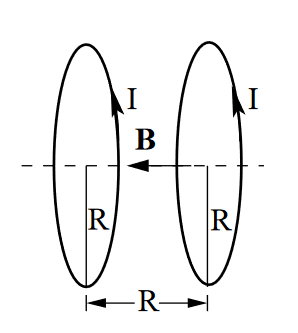
\includegraphics[height=5cm]{Screenshot (2)}
  \caption{Anordnung der Helmholtz-Spulen. \cite[S. 1]{kent}}
  \label{fig:drill}
\end{figure}


\begin{figure}[H]
  \centering
  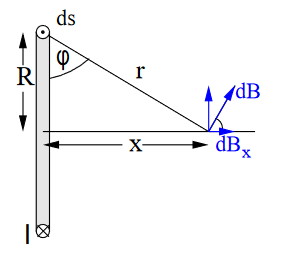
\includegraphics[height=5cm]{Screenshot (6)}
  \caption{Magnetfeld einer Spule im Zentrum der Helmholtz-Spulen. \cite[S. 1]{kent}}
  \label{fig:drill}
\end{figure}

\noindent Der Feldgradient 
\begin{equation}
    \frac{dB}{dx} = -3\mu_\text{0}IR^2 \frac{x}{(R^2+x^2)^{5/2}}
\end{equation}

\noindent ist in einem großen Bereich vernachlässigbar.




\subsection{Theorie zur Bestimmung des magnetischen Moments unter Ausnutzung der Gravitation}
Wirkt auf eine Masse $m$ die Gravitationskraft $\vec{F} = m \vec{g}$ , stellt sich ein Drehmoment $\vec{D}_\text{g}= m (\vec{r} \times \vec{g}) $ ein.
Entgegen der Gravitationskraft wirkt das Magnetfeld der Spulen. Ein Gleichgewicht zwischen Drehmoment $\vec{D}_\text{B} = \vec{\mu}_\text{Dipol} \times \vec{B}$
 und Drehmoment $\vec{D}_\text{g}$ tritt nur auf, wenn eine bestimmte Magnetfeldstärke gemäß
\begin{equation}
   \vec{\mu}_\text{Dipol}\times\vec{B} = m \cdot (\vec{r}\times\vec{g})
\end{equation}
eingestellt ist. Hierbei sind $g$ und $B$ parallel zueinander, weshalb sich die Gleichung durch
\begin{equation}
    \mu_\text{Dipol}\cdot B = m r g
\end{equation}
ausdrücken lässt.

\subsection{Theorie zur Bestimmung des magnetischen Moments über die Schwingungsdauer eines Magneten}
Wird eine Billiardkugel in Schwingung versetzt, verhält sie sich im homogenen Magnetfeld wie ein harmonischer Oszillator.
Die Bewegungsgleichung für den Prozess lautet:

\begin{equation}
    - \bigl|\vec{\mu}_\text{Dipol} \times \vec{B}\bigr| = J_\text{K} \cdot \frac{d^2\theta}{dt^2}.
\end{equation}

\noindent Die quadrierte Schwingungsdauer

 \begin{equation}
   T^2 = \frac{4\pi^2 J_\text{K}}{\mu_\text{Dipol}} \frac{1}{B}
\end{equation}
ist die Lösung der Gleichung, woraus sich dann das magnetische Moment bestimmen lässt.

\subsection{Theorie zur Bestimmung des magnetischen Moments über die Präzession eines Magneten}
Ein Kreisel erfährt eine Präzessionsbewegung, wenn eine äußere Kraft auf die Drehachse eines rotierenden Körpers wirkt.
Die Drehachse bewegt sich hierbei auf dem Kegelmantel um die Drehimpulsachse.
Wird eine rotierende Billiardkugel ausgelenkt, bleibt die Auslenkung wegen der Rotation stabil.
Existiert außerdem ein Magnetfeld, wirkt eine äußere Kraft und die Präzessionsbewegung entsteht, welche durch
\begin{equation}
    \vec{\mu}_\text{Dipol} \times \vec{B} = \frac{d\vec{L}_\text{K}}{dt}
\end{equation}
beschrieben wird. Diesmal stellt die Präzessionsfrequenz
\begin{equation}
\Omega_\text{p} = \frac{\mu B}{\bigl|L_\text{K}\bigr|}
\end{equation}
eine Lösung dar. Der Drehimpuls kann über das Trägheitsmoment und dessen Kreisfrequenz bestimmt werden und das magnetische Moment folgt über:

\begin{equation}
\frac{1}{T_\text{p}} = \frac{\mu_\text{Dipol}}{2\pi L_\text{K}} B.
\end{equation}
